%\documentclass[10pt,a4paper]{article}
\documentclass[12pt,a4paper]{article}
\usepackage{graphicx,amsmath}
%\usepackage{subfigure}
\usepackage{float}
\usepackage[german]{babel}
\usepackage[utf8]{inputenc}
\setcounter{secnumdepth}{4}
\usepackage[top=2cm, bottom=2.5cm, left=3cm, right=3cm]{geometry}
\usepackage{subcaption}
\begin{document}

\begin{figure}[H]
	\centering
	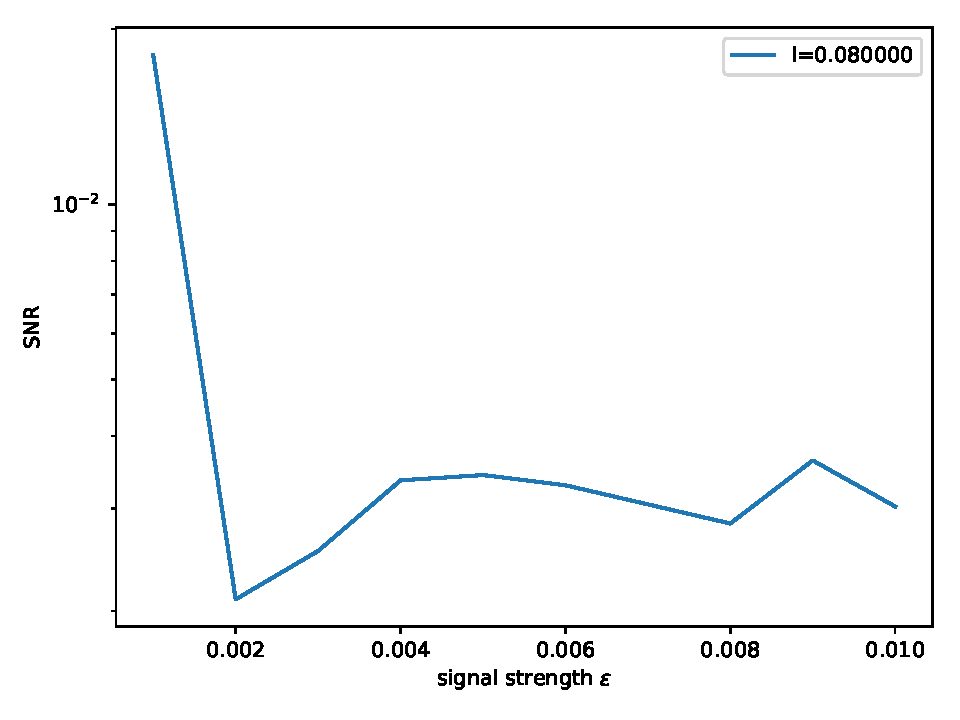
\includegraphics[scale=0.9]{snrepsautorealdrange6aem2.pdf}
	\caption{Abhängigkeit des gemessenen SNR von der Signalstärke}
	\label{eps}
\end{figure}
\end{document}